\documentclass{article}
\usepackage{graphicx}
\usepackage[hidelinks]{hyperref}
\usepackage{titlesec}
\usepackage{fancyvrb}
\usepackage{subcaption}
\captionsetup{compatibility=false}
\graphicspath{ {./images/} }
\titleformat{\chapter}{}{}{0em}{\bf\LARGE}
\titlespacing*{\chapter}{0pt}{40pt}{10pt}

\usepackage{geometry}
 \geometry{
 a4paper,
 total={170mm,257mm},
 left=20mm,
 top=20mm,
 }

\usepackage{etoolbox}
\makeatletter
\patchcmd{\chapter}{\if@openright\cleardoublepage\else\clearpage\fi}{}{}{}
\makeatother

\title{
\includegraphics[width=8cm]{bashlogo.png} \\[2cm] CS 108 - Bash Grader}
\author{Siddhant Mulkikar}
\date{\today}

\begin{document}

\maketitle
\newpage
\tableofcontents
\newpage

\section{Objective}
The objective of this CS108 Project was to create a csv file manager and interpreter with a command line interface.

\section{Introduction}
Bash Grader is a command line interface for instructors to grade students and manage their marks. It is an incredibly useful tool with its many functionalities and features. 

\section{List of Functionalities}
\subsection{Basic functionalities}
\begin{itemize}
    \item Upload a marklist in the form of a csv file.
    \item Total the marks of each student over all exams
    \item Combine the marks of all exams into a single csv file
    \item Update the marks of a student in a particular exam
\end{itemize}
\newpage
\section{Usage}
\subsection{Upload}
Run the following command to upload a csv file in your current directory.
\begin{verbatim}
    bash submission upload <filename>
\end{verbatim}


\subsection{Total}
Run the following command to total the marks of each student over all exams into a total column in \verb"main.csv".
\begin{Verbatim}
    bash submission total
\end{Verbatim}


\subsection{Combine}
The following command combines all the csv files in the current directory into \verb"main.csv".
\begin{Verbatim}
    bash submission combine
\end{Verbatim}


\subsection{Update}
Run the following command to update the marks of a particular student
\begin{verbatim}
    bash submission update
\end{verbatim}

\newpage

\section{Working}
\subsection{Upload}
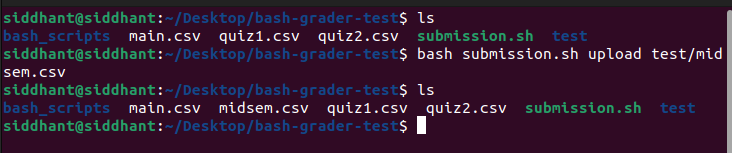
\includegraphics[width=\textwidth]{upload.png}
In the above example, the file \verb"quiz1.csv" is uploaded i.e. copied into the current directory from the filepath given as argument by the user.
The script checks if the file exists and if it is a csv file. If it is, only then is the file copied into the current directory.\\
\textbf{Script files : upload.sh }


\subsection{Total}
\begin{center}
    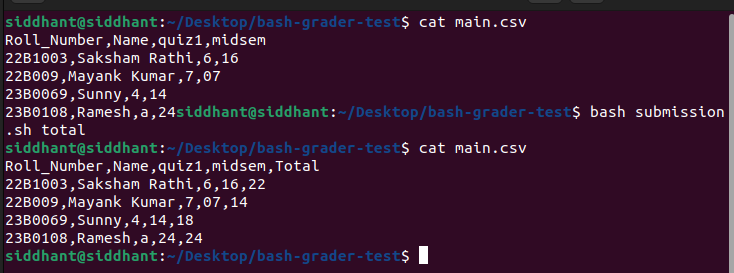
\includegraphics[width=10cm]{total.png}
\end{center}
In the above example, the script totals the marks of each student over all exams and adds a new column \verb"Total" to the \verb"main.csv" file.
If the marks column has \verb"a" as its entry, the script skips that row while totaling.\\
\textbf{Script files : total.awk }

\subsection{Combine}
\begin{figure}[h]
    \begin{subfigure}{0.5\textwidth}
    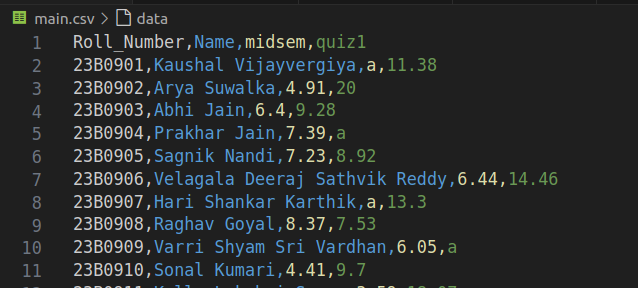
\includegraphics[width=\linewidth, height=3cm]{before_combine.png} 
    \caption{Before combine}
    \label{fig:subim1}
    \end{subfigure}
    \begin{subfigure}{0.5\textwidth}
    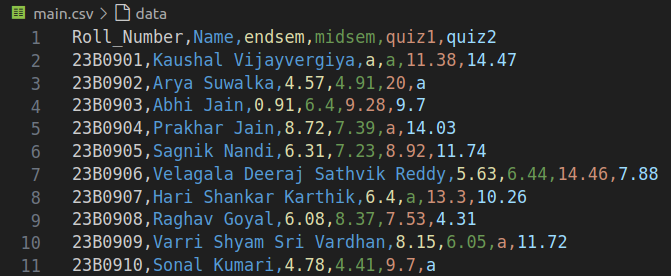
\includegraphics[width=\linewidth, height=3cm]{after_combine.png}
    \caption{After combine}
    \label{fig:subim2}
    \end{subfigure}
\end{figure}
In the above example, the script combines all the csv files in the current directory into a single \verb"main.csv" file. The script checks if the file is a csv file and if it is not the \verb"main.csv" file.\\ \verb"main.csv" is constructed from scratch in the following steps:
\begin{enumerate}
    \item First, an array of all unique roll numbers and names is created.
    \item Then, based on the exam files, a header is created with the roll numbers and names.
    \item A mesh of \verb"a"'s is created with the dimensions of the header.
    \item Then the script iterates over all exam files and fills in the marks of each student in the mesh, whenever they are found. This ensures that anyone who is not present in a particular exam file is marked as \verb"a"(absent) in \verb"main.csv" for that particular exam.
\end{enumerate}
\hfill
\textbf{Script files : combine.sh combine.awk}
\newpage

\subsection{Update}
\begin{figure}[h]
    \begin{subfigure}{0.5\textwidth}
    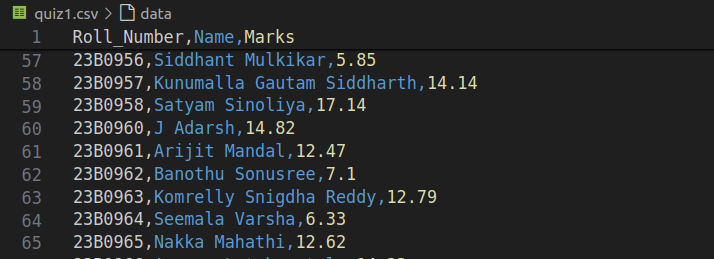
\includegraphics[width=\linewidth, height=3cm]{quiz-before.png} 
    \caption{quiz1.csv before update}
    \end{subfigure}
    \begin{subfigure}{0.5\textwidth}
    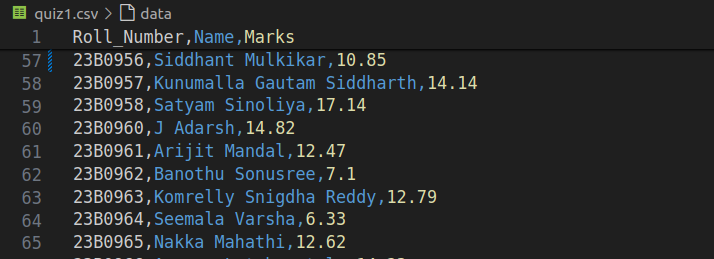
\includegraphics[width=\linewidth, height=3cm]{quiz-after.png}
    \caption{quiz2.csv after update}
    \end{subfigure}
\end{figure}
\begin{figure}[h]
    \begin{subfigure}{0.5\textwidth}
    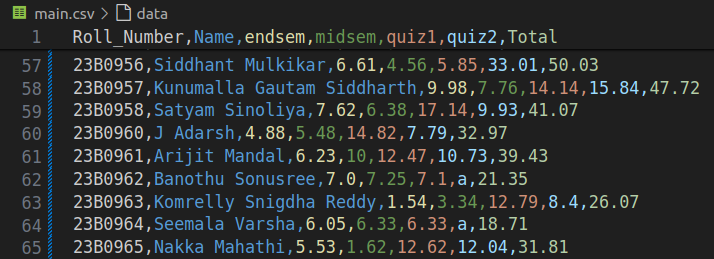
\includegraphics[width=\linewidth, height=3cm]{main-before.png} 
    \caption{main.csv before update}
    \end{subfigure}
    \begin{subfigure}{0.5\textwidth}
    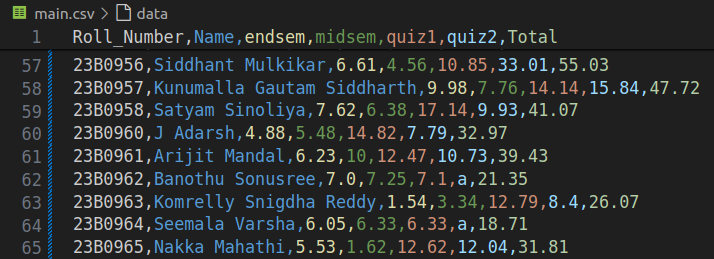
\includegraphics[width=\linewidth, height=3cm]{main-after.png}
    \caption{main.csv after update}
    \end{subfigure}
\end{figure}
In the above example, the script updates the marks of \textbf{23B0956} in \verb"quiz1.csv" and \verb"main.csv".\\
The script first checks if the student is present in the \verb"main.csv" file and if the exam file exists. If the student is present in the \verb"main.csv" file, the script updates the marks of the student in \verb"main.csv" by calling \verb"update_main.awk" and the exam file by calling \verb"update_exam.awk".\\
It also asks the user if they want to update the marks of the student in some other exam and repeats the same process. If the user does not want to update the marks of the student in any other exam, the script checks if \verb"main.csv" had been totaled before. If it was, then the script calls \verb"total.awk" to correct the total, as the marks in \verb"main.csv" have been updated.\\
\textbf{Script files : update.sh update\_exam.awk update\_main.awk total.awk} 
\end{document}
